\chapter{Microphone and Sampling}
%en eller anden indledning til dette afsnit

\section{Microphone}
In this project an electret microphone is used, since this is the one that is found in telephones. 
Microphones are used to convert sound into an electric signal. This is done by converting oscillations in the air into an oscillating voltage signal. 

\begin{figure}[H]
    \centering
    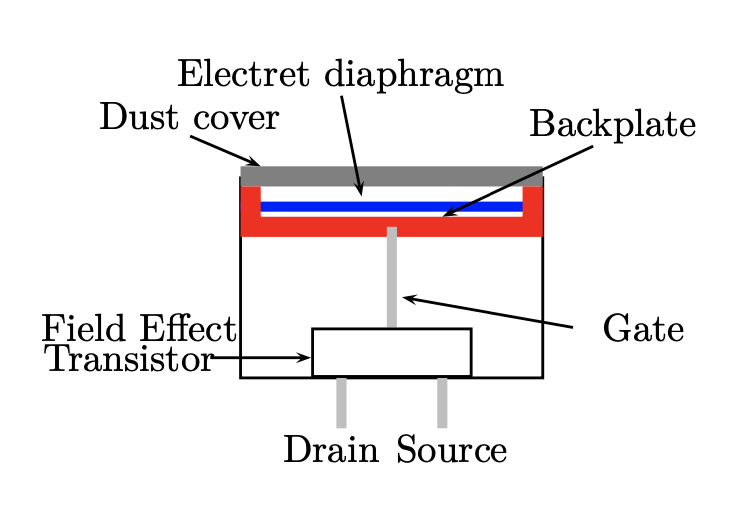
\includegraphics[scale=0.65]{figures/Microphone_figure.png}
    \caption{A figure of an electret microphone \cite[p. 160]{LectureNotes}}
    \label{fig:mic_figure}
\end{figure}

\autoref{fig:mic_figure} is a simpler version of a electret microphone. The electret microphone works when a signal is going through the dust cover and the electret diaphragm will begin to oscillate. When this happens there will be a change in distance between the backplate and the oscillating diaphragm. When this distance changes the capacitance changes and thus will the charge that were on the backplate. There will then be a change in voltage between the diaphragm and the backplate and this is detected by the field effect transistor (FET). The FET can also amplify the voltage. \\

\noindent The diaphragm and the backplate creates a capacitor with a capacitance, this can be described by:
$$ C = \dfrac{\varepsilon A}{d}$$ 
\indent where $\varepsilon$ is the permittivity (a measure of the electric polarisation of the electrical insulator), $A$ is the area of the plates and $d$ is the distance between the diaphragm and the backplate. $A$ and $\varepsilon$ is considered constants. $d$ can be described by letting $z(t)$ be the distance between the diaphragm and the backplate to time $t$, by doing this $C$ then becomes a function of $z$. The voltage between the plates and their charge has the relation:
$$q=C v_C.$$
This can also be described as:
$$v_C(t)=v_C(z(t))= \dfrac{q(t)}{C(z(t))} = \dfrac{q(t)z(t)}{\varepsilon A},$$
\indent where $v_C$ is the voltage between the plates. This means that when $z$ decreases, the distance between the plates becomes smaller, the charge on the diaphragm induces an increased charge on the backplate. 
\cite[p. 160-161]{LectureNotes}

%Skal der skrives mere til denne? er det nødvendigt at beskrive mechanical forces og electric forces? 

\section{Sampling}
\begin{figure} [H]
    \centering
    \begin{tikzpicture}[
    node distance = 7mm and -3mm,
every node/.style = {draw=black, rounded corners, fill=gray!30, 
                     minimum width=2cm, minimum height=0.5cm,
                     align=center},
every path/.style = {draw, -latex}
                        ]
\node (Actuators) {Actuators};
\node (Computation) [below  left=of Actuators]       {Computation}; 
\node (Sensor) [below right=of Computation]     {Sensor};
\node (Reality) [below right=of Actuators]     {Reality};

\draw   (Computation) |- (Actuators);
\draw   (Actuators) -| (Reality);
\draw   (Reality) |- (Sensor);
\draw   (Sensor) -| (Computation);
    \end{tikzpicture}
    \caption{Reality to computing} %better caption
    \label{fig:reality_computing}
\end{figure}
When working with signals an essential thing is to look at sampling. By sampling a signal it can then be stored analysed in a digital computer. From the figure \ref{fig:reality_computing}, sampling is necessary to come from sensor part to the computing part.  \\ 

\subsection{Discrete-time Signals}
In this project music signals are used which are continuous-time signals. Going from a continuous-time signal, $x_c(t)$, to a discrete-time signal,$x[n]$, the new discrete-time signal can be manipulated by a computer. A discrete-time signal i essentially a sampled continuous-time signal. The discrete-time signal is formally written as:
$$x={x(n)}, \quad    n \in Z$$
A typical way to obtain a discrete-time signal from a continuous-time signal is by using periodic sampling. A periodic sampling is a sequence of samples, $x[n]$, also referred to as the nth sample, obtained from the continuous-time signal,$x_c(t)$, by using the following relation:
$$x[n]=xc (nT), \quad    - \infty <n< \infty$$

where $T$ is the sampling period and it is from the relation $f=\dfrac{1}{T}$, where $f$ is the sampling frequency, in samples per second. This can also be called a C/D converter, ideal continuous to discrete converter. 
By using a A/D converter, analog to digital converter, an approximation of the C/D conversion is achieved. \cite[p. 140-142]{DiscreteTimeSignal}\\


\textbf{Hvad der mangler, ved dog ikke hvor meget af det er nødvendigt at skal have med, om vi overhovedet bruger det.} 
\begin{itemize}
    \item A/D conversion
    \begin{itemize}
        \item Bits needs to be explained
    \end{itemize}
    \item Modeling the process
    \begin{itemize}
        \item Dirac Delta
        \item Unit impulse response
    \end{itemize}
    \item Sample rate (uses Fourier as example)
    \item Aliasing (DFT)
    \item Quantization
\end{itemize}